\section{Requirements}

\subsection{Overall Requirements Specification}

\subsection{Selected Detailed Requirements}

\subsubsection{Functional \& Non-Functional Requirements}

\subsubsection{The Physical Setup (The Brewery Machine)}

\subsubsection{The Simulator}


\subsection{Use Cases}
Use cases are written descriptions of how a user will perform different tasks
on a system. They outline a systems behaviour as it responds to a request from
the user. Each use case is represented as a sequence of steps, beginning with
the users goal and ending when it that goal is fulfilled. \\

The first step in developing use cases is to determine the actors.


% \begin{table}[ht]
%    \begin{tabularx}{\textwidth}{|>{\RaggedRight}p{3cm}|>{\RaggedRight}X|>{\RaggedRight}p{2.5cm}|}
%     \hline
%     \textbf{Use Case ID}   & \textbf{Name}                                 & \textbf{Definition}\\ \hline
%     UC01                   & Start production line                         & User \\ \hline
%     UC02                   & Stop production line                          & User \\ \hline
%     UC03                   & Monitor and store data from production line   & SCADA \\ \hline
%     UC04                   & Monitor and display relevant data live        & SCADA \\ \hline
%     UC05                   & Create batch report                           & MES \\ \hline
%     UC06                   & Calculate OEE                                 & MES \\ \hline
%     UC07                   & Estimate the error function                   & MES \\ \hline
%     UC08                   & Find optimal production speed                 & MES \\ \hline
%     \end{tabularx}
%     \caption{Use Cases}
%     \label{table:use_cases}
%     \end{table}

\subsubsection{Actor List}
In order to determine who will be able to access the system, the actors are
found. An actor is defined as any external system or user that communicates
with the system. Not every actor can necessarily be found at the given time,
meaning other actors may be found later during development.

The identified actors can be seen in table \ref{table:actor_list}. With these
actors, a visualisation can be made, depicting how the different actors
communicate with the system.

\begin{table}[ht]
     \begin{tabularx}{\textwidth}{|>{\RaggedRight}p{2.5cm}|>{\RaggedRight}p{8cm}|>{\RaggedRight}X|}
     \hline
     \textbf{Actor} 				& \textbf{Description}                                                                                                              				& \textbf{Goal} \\ \hline
     \multirow{2}{*}{User (p)}      & The user represents the worker of the machine. The user will use the control panel to control the machine.                                  		& 	\begin{itemize}
     																																														\item Control machine
     																																														\item Start new batches
     																																													\end{itemize} \\ \hline
     \multirow{2}{*}{BPM (s)}     	& The beer production machine is responsible for supplying data to the MES and producing the beer.       											& \begin{itemize} 
     																																														\item Collect and save data
     																																														\item Communicate between hardware and MES 
     																																									 				\end{itemize} \\ \hline
    \end{tabularx}
    \caption{Actor list}
    \label{table:actor_list}
\end{table}

\subsubsection{Detailed Use Cases}
When the actors have been determined, use cases can be developed. These use
cases add value because they help explain how the system behaves and which
functions to include when developing the system. As seen below, in table
\ref{table:usecase_start}, which represents the sequence of steps happening
when a user wants to start the beer production machine. This use case clarifies
the functions needed to fulfil the users goal, to start the production machine.

% start production
\begin{table}[ht]
    \begin{tabularx}{\textwidth}{|>{\RaggedRight}X|}
        \hline
        \textbf{ID:} UC01  \\
        \hline
        \textbf{Primary actor:} The user \\
        \hline
        \textbf{Secondary actor:} Beer production machine \\
        \hline
        \textbf{Short description:} The MES must be able to start the brewery's
        production \\
        \hline
        \textbf{Pre conditions:} The beer production machine needs to be in
        ready mode, that is, not producing beer. \\
        \hline
        \textbf{Main flow:} \\
        	1. This use case starts when a user wants to start the beer
        	production machine. \\
        	2. The user chooses what kind of beer to be produced. \\
        	3. The user sets production speed. \\
        	4. The user sets batch id. \\
        	5. The user sets amount of beers to be produced. \\
        	6. The user presses the start button. \\
        	7. The MES starts the machine. \\
        	8. When the production has finished, the MES stores data from the
        	production. \\

		\hline
        \textbf{post conditions:} The beer production machine is turned on \\
        \hline
        \textbf{Alternative flow:} \\
        	Step 8: If the machine does not complete the production (for various
        	reasons) the production stops and stores the data from the machine
        	and the user receives an error message. \\
        \hline
    \end{tabularx}
    \caption{Production Control: Start machine}
    \label{table:usecase_start}
\end{table}

%% BELOW USE CASES BELONGS IN APPENDIX, IF PAGENUMBERS ALLOW IT
% % stop production
% \begin{table}[ht]
%     \begin{tabularx}{\textwidth}{|>{\RaggedRight}X|}
%         \hline
%         \textbf{ID:} UC02  \\
%         \hline
%         \textbf{Primary actor:} The user \\
%         \hline
%         \textbf{Secondary actor:} Beer production machine \\
%         \hline
%         \textbf{Short description:} The MES must be able to stop the brewery's
%         production \\
%         \hline
%         \textbf{Pre conditions:} The beer production machine needs to be on \\
%         \hline
%         \textbf{Main flow:} \\
%         	1. This use case starts when a user wants to shut down the beer
%         	production machine. \\
% 			2. The user presses the stop button \\
% 			3. The MES stores the data from the beer production machine \\
% 			4. The beer production machine stops \\
% 		\hline
%         \textbf{post conditions:} The beer production machine is turned off \\
%         \hline
%         \textbf{Alternative flow:} \\
%         \hline
%     \end{tabularx}
%     \caption{Production Control: Stop production} 
%     \label{table:usecase_stop}
% \end{table}

% % abort
% \begin{table}[ht]
%     \begin{tabularx}{\textwidth}{|>{\RaggedRight}X|}
%         \hline
%         \textbf{ID:} UC03  \\
%         \hline
%         \textbf{Primary actor:} The user \\
%         \hline
%         \textbf{Secondary actor:} Beer production machine \\
%         \hline
%         \textbf{Short description:} The MES must be able to abort the current
%         production. \\
%         \hline
%         \textbf{Pre conditions:} The production needs to be on and producing
%         beer. \\
%         \hline
%         \textbf{Main flow:} \\
%         	1. This use case starts when a user wants to abort the current
%         	production. \\
%         	2. The user presses the abort button \\
% 			3. The MES stores the data from the beer production machine \\
% 			4. The beer production machine aborts \\
% 		\hline
%         \textbf{post conditions:} The beer production machine aborted the
%         current production \\
%         \hline
%         \textbf{Alternative flow:} \\
%         \hline
%     \end{tabularx}
%     \caption{Production Control: Abort the current production} 
%     \label{table:usecase_abort}
% \end{table}

% % reset
% \begin{table}[ht]
%     \begin{tabularx}{\textwidth}{|>{\RaggedRight}X|}
%         \hline
%         \textbf{ID:} UC04  \\
%         \hline
%         \textbf{Primary actor:} The user \\
%         \hline
%         \textbf{Secondary actor:} Beer production machine \\
%         \hline
%         \textbf{Short description:} The MES must be able to reset the beer
%         production machine. \\
%         \hline
%         \textbf{Pre conditions:} The beer production machine needs to be in
%         ready mode, that is, not producing beer. \\
%         \hline
%         \textbf{Main flow:} \\
%         	1. This use case starts when a user wants to reset the beer
%         	production machine \\
%         	2. The user presses the reset button \\
% 			3. The beer production machine resets \\
% 		\hline
%         \textbf{post conditions:} The beer production machine has been reset \\
%         \hline
%         \textbf{Alternative flow:} \\
%         \hline
%     \end{tabularx}
%     \caption{Production control: Reset the machine}
%     \label{table:usecase_reset}
% \end{table}

% % clear
% \begin{table}[ht]
%     \begin{tabularx}{\textwidth}{|>{\RaggedRight}X|}
%         \hline
%         \textbf{ID:} UC05  \\
%         \hline
%         \textbf{Primary actor:} The user \\
%         \hline
%         \textbf{Secondary actor:} The beer production machine \\
%         \hline
%         \textbf{Short description:} The MES must be able to clear the beer
%         production machine. \\
%         \hline
%         \textbf{Pre conditions:} The beer production machine needs to be in
%         ready mode, that is, not producing beer. \\
%         \hline
%         \textbf{Main flow:} \\
%         	1. This use case starts when a user wants to clear the beer
%         	production machine \\
%         	2. The user presses the clear button \\
% 			3. The beer production machine clears \\
% 		\hline
%         \textbf{post conditions:} The beer production machine has been cleared \\
%         \hline
%         \textbf{Alternative flow:} \\
%         \hline
%     \end{tabularx}
%     \caption{Production control: Clear the machine}
%     \label{table:usecase_clear}
% \end{table}

% % display live data
% \begin{table}[ht]
%     \begin{tabularx}{\textwidth}{|>{\RaggedRight}X|}
%         \hline
%         \textbf{ID:} UC06  \\
%         \hline
%         \textbf{Primary actor:} The user \\
%         \hline
%         \textbf{Secondary actor:} The beer production machine \\
%         \hline
%         \textbf{Short description:} The MES needs to display live data from the
%         production. \\
%         \hline
%         \textbf{Pre conditions:} The beer production machine needs to be on and
%         producing beer. \\
%         \hline
%         \textbf{Main flow:} \\
%         	1. This use case starts when the user wants to see data from the
%         	production. \\
% 			2. The MES collects the necessary data from the beer production
% 			machine. \\
% 			3. The MES displays the relevant data for the user. \\
% 		\hline
%         \textbf{post conditions:} Live data has been displayed for the user. \\
%         \hline
%         \textbf{Alternative flow:} \\
%         \hline
%     \end{tabularx}
%     \caption{Production monitoring: Display live data}
%     \label{table:usecase_displayLiveData}
% \end{table}

% % generate batch report
% \begin{table}[ht]
%     \begin{tabularx}{\textwidth}{|>{\RaggedRight}X|}
%         \hline
%         \textbf{ID:} UC07  \\
%         \hline
%         \textbf{Primary actor:} The user \\
%         \hline
%         \textbf{Secondary actor:} The beer production machine \\
%         \hline
%         \textbf{Short description:} The MES needs to be able to generate a batch
%         report from previous batches. \\
%         \hline
%         \textbf{Pre conditions:} The beer production machine needs to have
%         produced a batch. \\
%         \hline
%         \textbf{Main flow:} \\
%         	1. This use case starts when the user wants to see a batch report
%         	from previous productions. \\
% 			2. The MES generates a batch report \\
% 			3. The MES displays the batch report to the user. \\
% 		\hline
%         \textbf{post conditions:} A batch report has been displayed for the
%         user. \\
%         \hline
%         \textbf{Alternative flow:} \\
%         \hline
%     \end{tabularx}
%     \caption{Batch report: Generate batch report}
%     \label{table:usecase_batchReport}
% \end{table}

\subsubsection{Use Case Diagram}
Below, in figure \ref{figure:ucdiagram}, an overview of the use cases for the
MES can be seen.

\begin{figure}[ht]
	\centering 
	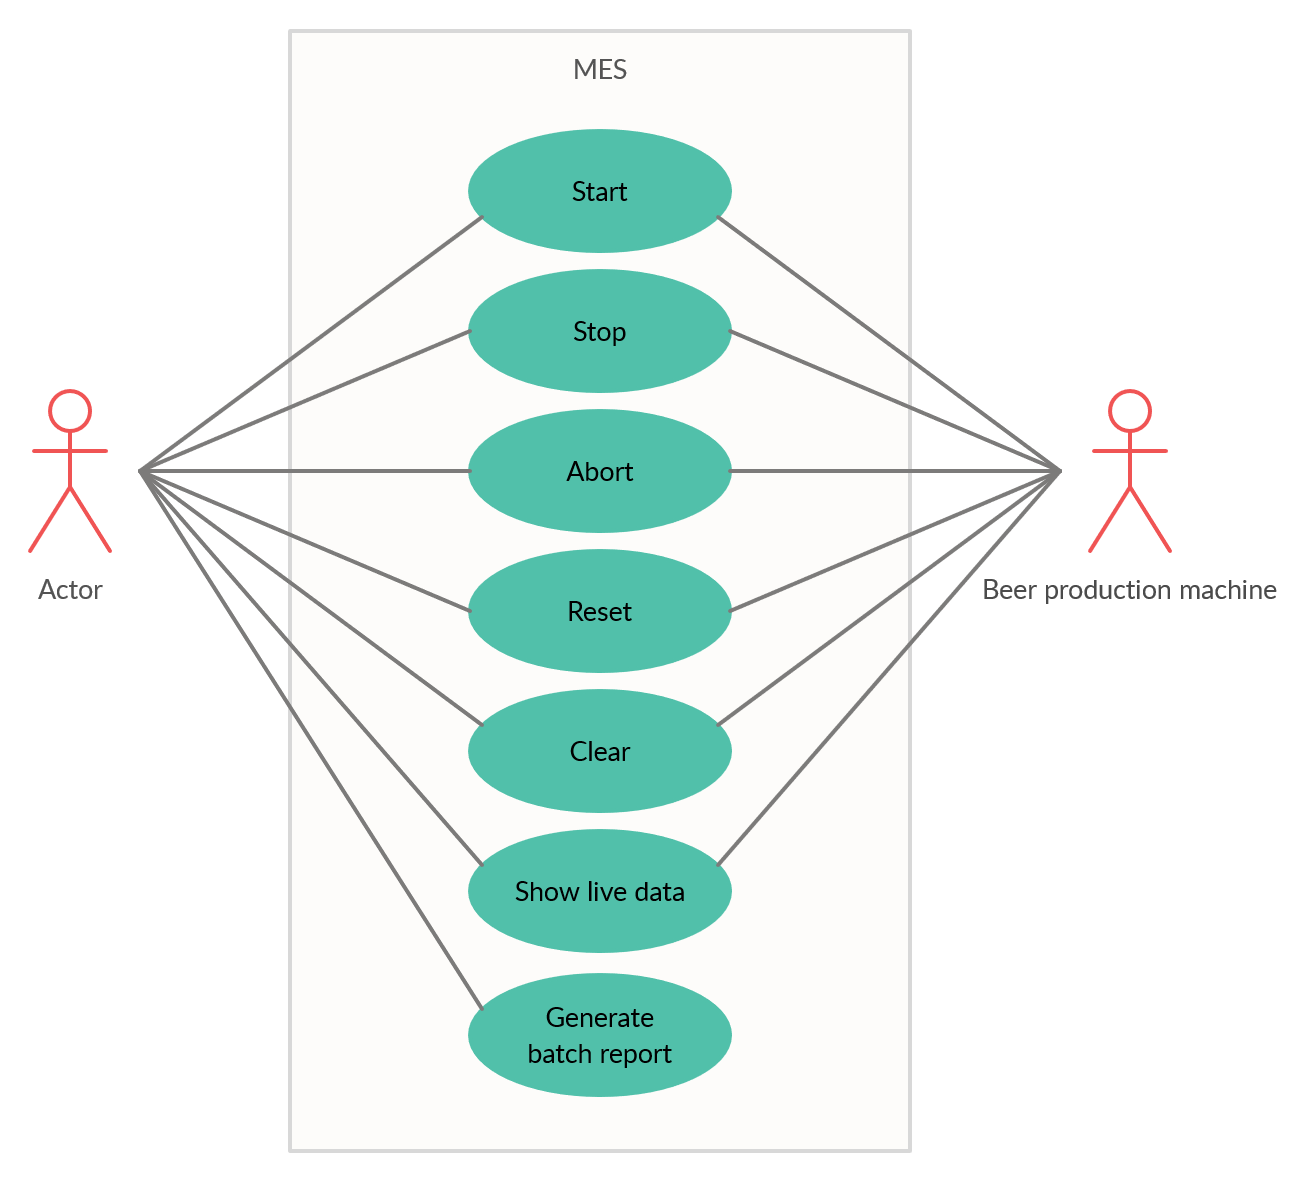
\includegraphics[scale=0.3]{images/ucdiagram.png}
	\caption{Use case diagram}
	\label{figure:ucdiagram} 
\end{figure}